%!TEX root = ../Thesis.tex
%\chapter{Long chapter title with $\pi$ $π$ or π}
%\chapter{Long chapter title with \texorpdfstring{$\pi$ $π$ or π}{π π or π}}
\section[Gaussian Mixture Models for Robust Unsupervised Scanning-Electron Microscopy Image Segmentation of North Sea Chalk]{Gaussian Mixture Models for Robust Unsupervised Scanning-Electron Microscopy Image Segmentation of North Sea Chalk}

\paragraph{Abstract:} Scanning-Electron images from North Sea Chalk are studied for important rock properties. To relieve this manual labor, we investigated several standard image processing methods that underperformed on complicated chalk. Due to the lack of manually labeled data, deep neural networks could not be adequately applied. Gaussian Mixture Models learnt a two-fold representation that separated the background well from the rock. Subsequent morphological filtering cleans up the prediction and enables automatic analysis. 

{\vfill\hfill\newline\fbox{\parbox{.97\textwidth}{\fullcite{dramsch2018gaussian}}}}
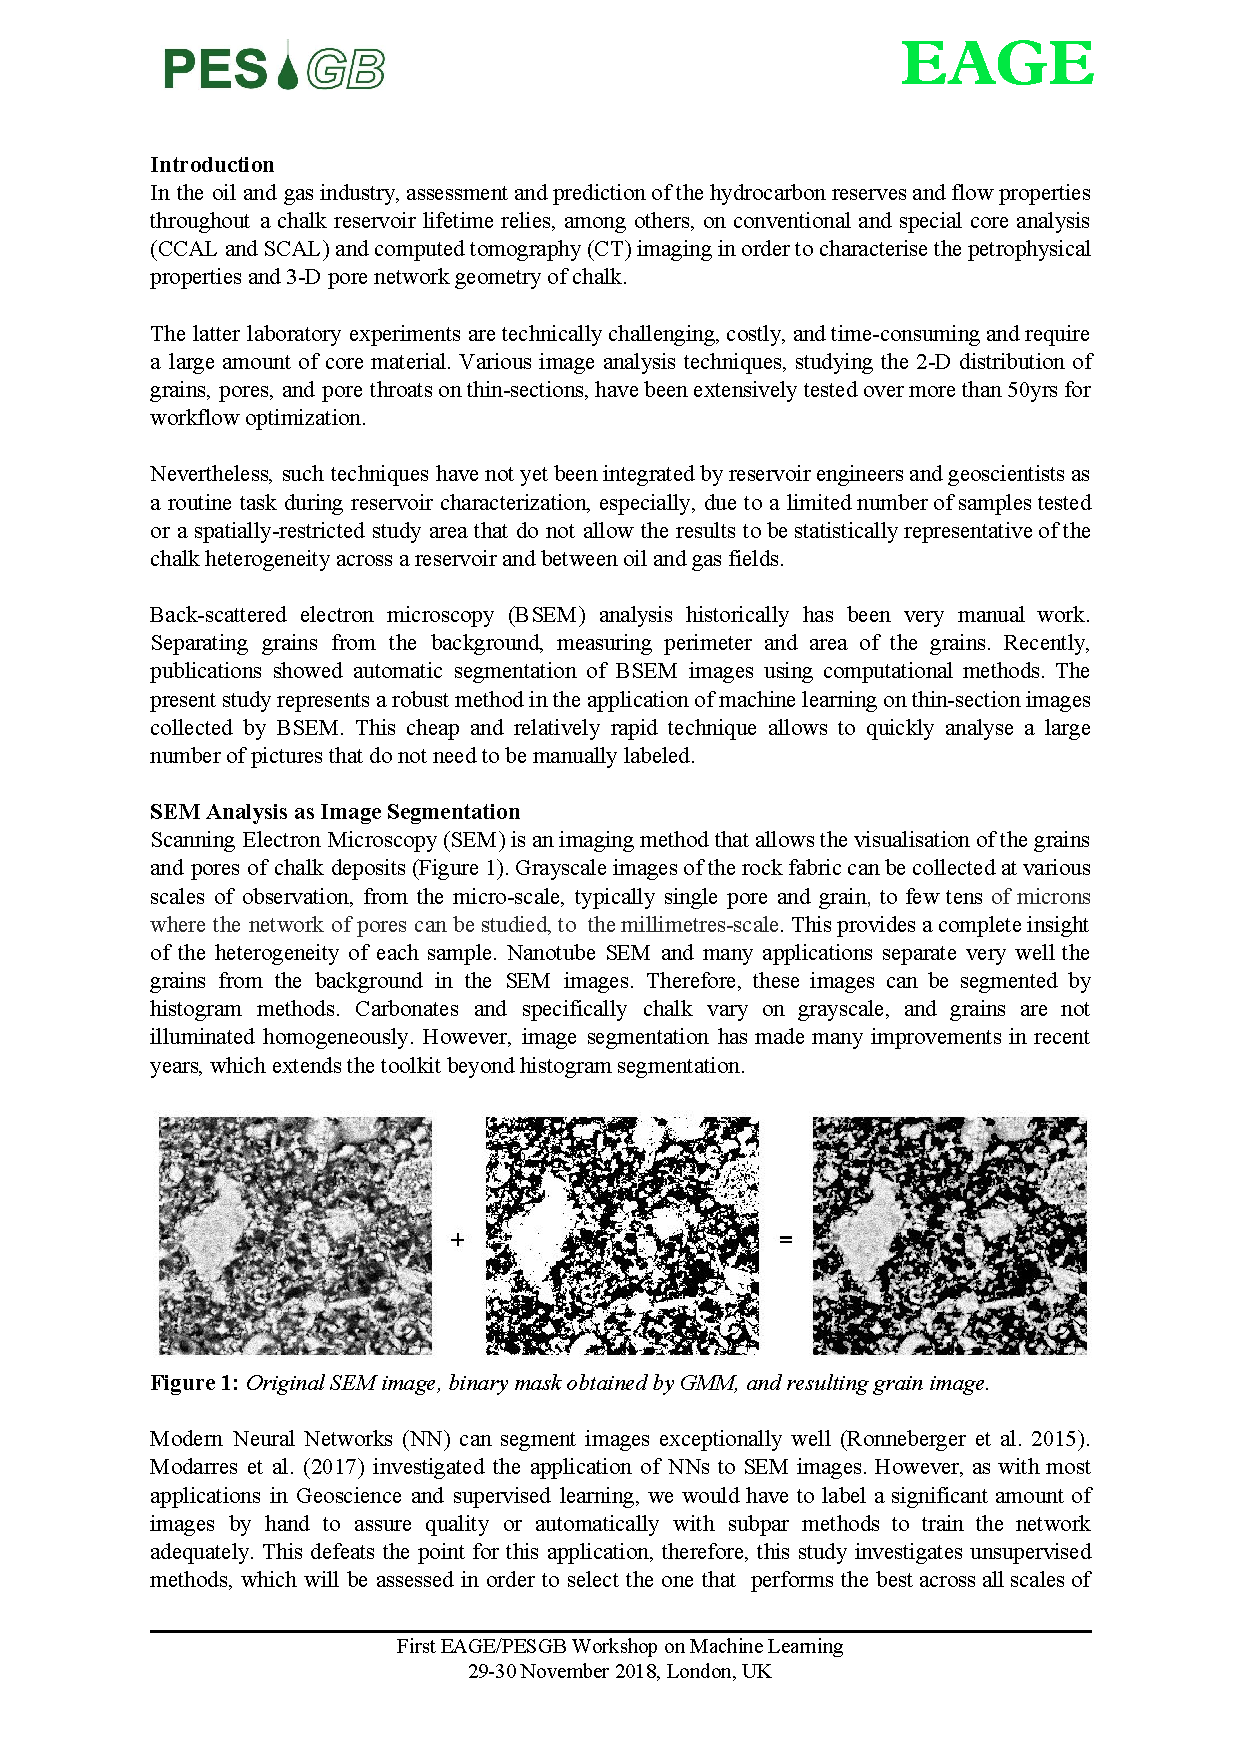
\includepdf[pages=1-2,pagecommand={},width=1.2\textwidth,offset=0.7cm -1.5cm]{papers/2018.2}